% !TEX root = ../main.tex


\chapter{Background}


In the dynamic landscape of cryptocurrencies, ensuring transparency, accountability, and financial stability
is paramount for marketplaces. This section provides an overview of the concepts and mechanisms
necessary to follow along the conception of a daily proof of liabilities. We explore the various approaches adopted by leading exchanges
to demonstrate their financial health through proof of reserves or solvency mechanisms. Additionally, we
highlight the shortcomings and challenges associated with current solvency verification practices, mainly the lack of recurrent proof of reserves,
paving the way for a daily proof in the subsequent sections.


\section{Bitcoin}
Bitcoin is recognized as the world's first successful cryptocurrency and decentralized digital currency.
The goal of Bitcoin is to allow financial transactions to be settled on their own, without the need of a middleman, typically financial institutions.
Bitcoin is built on a peer-to-peer network, which means that every participant helps in safe keeping the transactions history, and propagating the new transactions.
There is no single point of failure. This allows for transactions to occur in real time, in contrast to the delays encountered in the traditional finance world.
Bitcoin defines two different concepts: Bitcoin the cryptocurrency, and Bitcoin the blockchain. The cryptocurrency resides on the blockchain.
The Bitcoin blockchain is a decentralized ledger that records all Bitcoin (the cryptocurrency) transactions immutably and transparently.
This blockchain serves as a verifiable record of all Bitcoin transactions, accessible to every participant in the network.
The transparency afforded by the public blockchain engenders trust and accountability. \cite{MB17}


\subsection{Transactions}
For every participant of the network, there is a public key, a private key and a wallet address associated with the participant.
The public key is derived from the private key using elliptic curve multiplication, and the wallet address is derived from the public key using a hashing function.
Both are one way functions, meaning you cannot derive the other way around.
The public key serves as the unique identifier in the network, but it is the wallet address that typically defines a participant.
The wallet address can be seen as a bank account number. When you send Bitcoin to someone, you send it to their wallet address.
To be able to send some Bitcoin, you need to create a transaction and send it to the network.
When transactions are sent on the network, there is no way of knowing who propagated the transaction first.
We need to make sure a transaction originates from the sender. The way to do that is to sign your transaction. The digital signature is created from the transaction data and the private key, which is only known by the owner of the address.
The digital signature is created using the ECDSA (Elliptic Curve Digital Signature Algorithm) over the secp256k1 curve, which is the specific elliptic curve used by Bitcoin.
We verify a Bitcoin transaction's digital signature by using the sender's public key to check that the signature matches the hashed transaction data.
This is done through ECDSA, where the signature is compared to a computed value derived from the transaction hash and the public key.
If they match, it confirms the transaction was signed with the corresponding private key, validating the transaction.
Sending a transaction is the easiest problem to solve. The real challenge is to keep track of who owns what, and to avoid the double spending problem.
The methodology for managing this is to keep the history of every single transaction. The transactions are bundled up into blocks, and the chain of blocks creates the blockchain. \cite{MB17}

\subsection{Network}
The challenge of the network is to have every single node achieve consensus on the transaction history. Nodes are computers connected to the network,
working on publishing new blocks. The nodes work collectively to establish order of transactions (sequencing). Every new transaction is broadcast to all nodes.
The nodes put the transactions into a block, and try to publish that block. In order to publish a block, each node needs to solve a proof-of-work challenge.
When a node solves the challenge, it broadcasts the block to every node. The node accepts the block if all transactions are valid. There is no formal
way of approving a new block. A node shows its acceptance by starting to work on a new block using the hash of the accepted block as previous hash.
Some nodes might accept different blocks, if multiple blocks are propagated at the same time. This would create multiple chains. To solve this issue, the longest chain is considered to be the correct one.
If two chains have the same length, nodes keep working on their respective chains until one of the chains receives a new block, breaking the tie. \cite{MB17}

\begin{figure}[H]
   \centering
   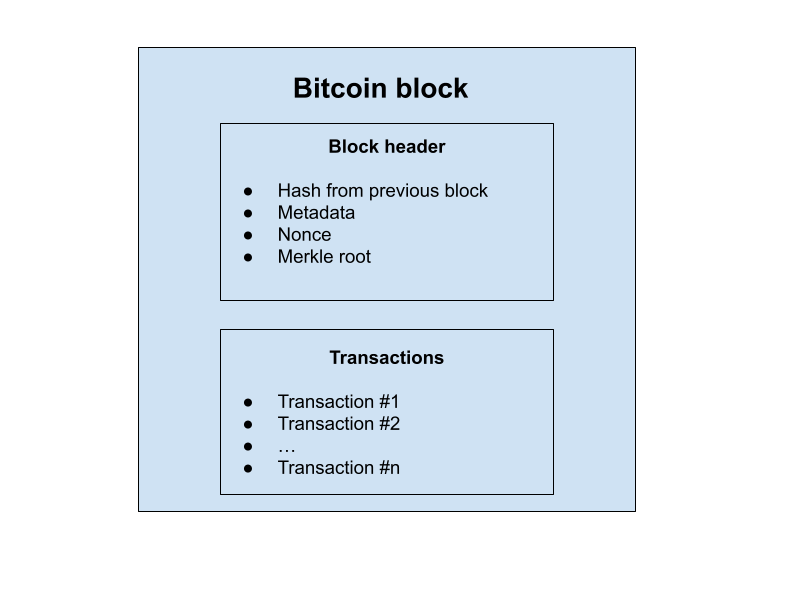
\includegraphics[width=130mm]{BitcoinBlock.png}
   \caption{Bitcoin block}
   \label{overflow}
   \end{figure}


\subsection{Proof-of-work}

In order to submit a new block, a node has to find a hash with a specific number of leading zeros.
The hash is produced by the SHA-256 algorithm and is 256 bits long, typically represented as a 64-character hexadecimal string. 
The number of leading zeros required is determined by the network's difficulty, which sets the target value that the hash must be less than or equal to for the block to be valid.
For instance, the threshold might be $0000000000000000abc123...$
This cryptographic puzzle serves as a barrier to entry, ensuring that a lot of computational power was spent on creating the block.
The way to test different hash values is to change the block timestamp, and the nonce value.
The nonce value is there solely for that purpose. Once a block is published, you cannot change any value inside of it because the hash value would change.
The immutability of the older blocks is what makes Bitcoin secure. To modify a block in the middle of the chain, you would need to redo the work of every single block made after that.
The longest chain is determined by the cumulative proof-of-work invested in it. This is why we say that Bitcoin is secure as long as $51\%$  of the nodes are honest.
The chain with the majority of nodes working on it will grow the fastest, thus will be the accepted chain.
The difficulty of the new block is determined by an average, in order to generate blocks at a steady pace. There is also a Bitcoin reward associated with mining (publishing) a block. \cite{MB17}


\subsection{Merkle Tree}
In the architecture of the blockchain, only the Merkle root is stored in the block header. Nodes only keep the recent blocks in memory. For the older blocks, they keep only the block header in memory.
This storage ensures the integrity of the blockchain, while decreasing the memory required to have the full blockchain history.
Since the hash of a block is the hash of the block header, this strategy does not impact the integrity checks of the blockchain.
The Merkle root is the top of the Merkle Tree, and is a unique identifier of the full tree. A Merkle tree is a tree where the parent node is the hash of the child nodes.
The tree is immutable because changing a single node would have an impact on the Merkle root.


\iffalse
\begin{figure}[ht!]
   \centering
   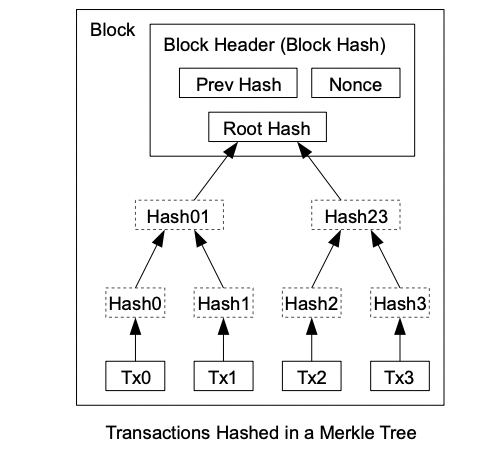
\includegraphics[width=90mm]{MerkleTree.png}
   \caption{Bitcoin Merkle Tree \cite{N08}}
   \label{overflow}
   \end{figure}
\fi


\section{Marketplaces}
The best way to buy Bitcoin for the first time is through marketplaces. Marketplaces facilitate the exchange of traditional currency for Bitcoin.
However, it's important to understand that the Bitcoin you purchase initially remains in the custody of the platform, rather than being sent directly to your personal wallet.
To gain custody of your Bitcoin, you need to request a transfer to your own wallet, similar to how traditional banking transactions rely on the bank to process your request.
Once you have Bitcoins in your wallet, you can transact on the network without needing a third party.
Unless you are running a node, you will need to trust a 3rd party, whether it is a marketplace, or over the counter, to first acquire Bitcoin.


When your Bitcoin is held in the marketplace's custody, it cannot be track onchain. It blends with the plarform's holdings.
Marketplaces manage many wallets, some public and some private, which enhances the privacy of deposits and withdrawals but contradicts Bitcoin's design for transparency and independence from third parties. 
This lack of visibility poses a challenge, as users have no proof of the marketplace's solvency to reimburse all clients. 
However, this issue is being addressed through the introduction of proof of solvency (or proof of reserve) mechanisms, 
which allow marketplaces to demonstrate their solvency. 
While this is a positive development, current proof of solvency methods have shortcomings and are not fully sufficient to prove solvency.


\section{Zero Knowledge}
Zero-knowledge proof is a cryptographic techniques that allow a prover to demonstrate knowledge of a fact without divulging any additional information. 
For instance, rather than revealing the solution to an equation, zero-knowledge proofs enable the prover to show that they know the solution without revealing it. 
In this context, a witness is the secret information or evidence that supports the validity of the statement being proven. 
The goal is to construct a proof that is both sound and complete, and is zero-knowledge \cite{LZK}.

\begin{itemize}
\item \textbf{Completeness}: If the statement is true, an honest verifier will be convinced by an honest prover.
\item \textbf{Soundness}: If the statement is false, no dishonest prover can convince the honest verifier (except with some infinitesimal probability).
\item \textbf{Zero-Knowledge}: If the statement is true,  a verifier learns nothing other than the fact that the statement is true. \cite{LC23}
\end{itemize}


\subsection{Non interactive proofs}

Zero knowledge proofs were originally designed as interactive, that is, multiple rounds of interaction between the prover and the verifier \cite{GMR89}.
leading to what are called interactive zero-knowledge proofs. This interaction allows the prover to demonstrate knowledge of the solution without revealing any additional information.
An alternative model was then proposed where the verifier and prover use a reference string that is shared during a trusted setup. Once we have the reference string, a single message is needed between the prover and the verifier.
The elimination of multiple rounds of interaction simplifies the verification process and reduces the computational power required.
Therefore, noninteractive zero-knowledge proofs offer enhanced efficiency and scalability, which will be needed later on.  \cite{BFM88} \cite{GMW91}


\subsection{SNARKS}
One of the recent advances for non-interactive proofs is what is known as SNARK (non-interactive argument of knowledge).
This means a proof that is:
\begin{itemize}
\item \textbf{Succinct}: The size of the proof is very small compared to the size of the witness.
\item \textbf{Non-interactive}: There are no rounds of interactions between the prover and the verifier.
\item \textbf{Argument}: It is secure only against provers with bounded computational resources. A dishonest prover with unlimited computational power could potentially prove a false statement.
\item \textbf{Knowledge-sound}: A valid proof can only be generated if the prover knows the witness. \cite{NZ20}
\end{itemize}

Moreover, a SNARK can also be zero-knowledge, where the prover demonstrates knowledge without revealing any additional information about the witness. We call such proof a zk-SNARK.
To be able to construct a SNARK, we need to transform the code we want to prove in a quadratic arithmetic program (QAP).


\subsubsection{Arithmetic circuit}
\label{subsec:ac}

Let's say we want to prove $x3+x+5=35$.
The Prover as to convince the Verifier that he knows the solution whitout revelaing it to him.

The first step of transforming a problem in the QAP form is to express a problem in the form of an arithmetic circuit.
An arithmetic circuit is a set of gates, each assigned a distinct set of inputs corresponding to the numbers to be processed in the operation.
These gates are configured to execute arithmetic operations such as addition, subtraction, multiplication, or division. The outputs of the gate circuit represent the digits of the resulting computation.

\begin{figure}[H]
   \centering
   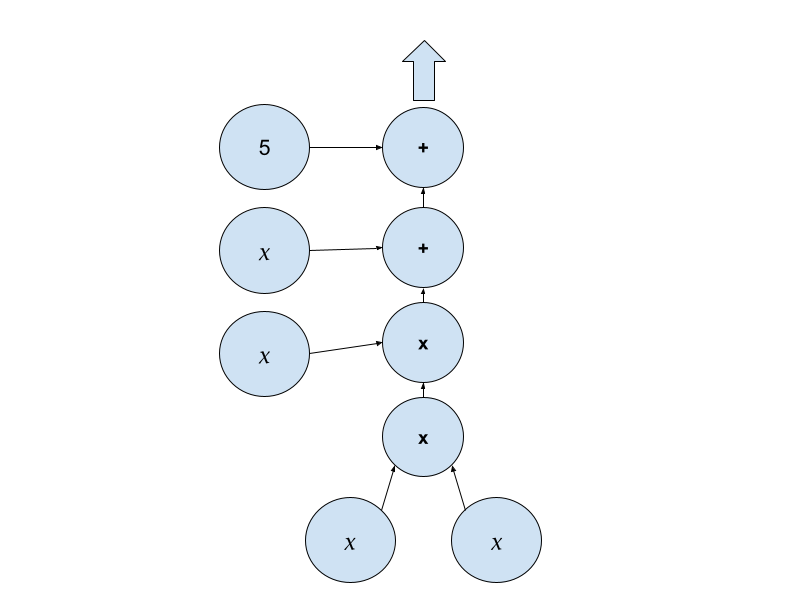
\includegraphics[width=130mm]{ArithmeticCircuit.png}
   \caption{General Arithmetic circuit}
   \label{overflow}
   \end{figure}

   \subsubsection{R1CS}
   The first step is to express our circuit as a set of constraint where each constraint contains only one arithmetic operation.
   \begin{quote}
   $s_1 = x * x$
   $s_2 = s_1 * x$
   $s_3 = s_2 * x$
   $~out = s_3 + 5$
   \end{quote}

   We can now convert this into an R1CS.
   An R1CS is a sequence of groups of three vectors $(a, b, c)$, where the solution to the R1CS is a vector $s$, and $s$ must satisfy the equation $s . a * s . b - s . c = 0$, where $.$ represents the dot product.
   The length of each vector is the length of the total number of variables for the system, including a variable $~one$ at the beginning, the variable $~out$, and all intermediate variables.
   The standard way of representing the three vectors $(a, b, c)$ is to create a mapping with the variables.
   Here is the mapping we will use:
   $'~one', '~out', 'x','s_1','s_2','s_3'$
   This gives us for the first gate:
   \begin{quote}
      $a = [0,0,1,0,0,0]$
      $b = [0,0,1,0,0,0]$
      $c = [0,0,0,1,0,0]$
   \end{quote}
   We are checking here that $x*x=s_1$.
   $a$ and $b$ both represents $x$, while $c$ represents $s_1$.

   Let's verify that our first gate satisfies the solution equation:
   $s . a * s . b - s . c = 0$
   We know that the solution to the equation is $ x = 3 $, so given that our $s$ vector
   would be: 
   \begin{quote}
   $s=[1,out,x,s_1,s_2,s_3]$
   $s=[1,35,3,9,27,30]$
\end{quote}

Now if we do the dot product:
\begin{quote}
   $s . a =  [1,35,3,9,27,30] . [0,0,1,0,0,0] = 0*1+0*35+1*3+0*9+0*27+0*30= 3$ 
   $s . b = [1,35,3,9,27,30] . [0,0,1,0,0,0] = 3$ 
   $s . c = [1,35,3,9,27,30] . [0,0,0,1,0,0] = 9$ 
$s . a * s . b - s . c =  3 * 3 - 9 = 0$

This shows that our solution vector satisfies the first gate.
\end{quote}

   Following these rules, our second gate for $s_1*x=s_2$ is:
   \begin{quote}
      $a = [0,0,0,1,0,0]$
      $b = [0,0,1,0,0,0]$
      $c = [0,0,0,0,1,0]$
   \end{quote}

   The third gate for $s_2+x=s_3$:
   \begin{quote}
      $a = [0,0,1,0,1,0]$ ($s_2+x$)
      $b = [1,0,0,0,0,0]$ ($1$)
      $c = [0,0,0,0,0,1]$ ($s_3$)
   \end{quote}

   4th gate for $s_3+5=~out$:
   \begin{quote}
      $a = [5,0,0,0,0,1]$
      $b = [1,0,0,0,0,0]$
      $c = [0,1,0,0,0,0]$
   \end{quote}
   
   The R1CS put together:
   \begin{quote}
      $
      A
      [0,0,1,0,0,0]
      [0,0,0,1,0,0]
      [0,0,1,0,1,0]
      [5,0,0,0,0,1]

      B 
      [0,0,1,0,0,0]
      [0,0,1,0,0,0]
      [1,0,0,0,0,0]
      [1,0,0,0,0,0]

      C 
      [0,0,0,1,0,0]
      [0,0,0,0,1,0]
      [0,0,0,0,0,1]
      [0,1,0,0,0,0]
      $
   \end{quote}
   \cite{RC23}

   \cite{VB16}
   
   
   \subsubsection{QAP}
   Next step is converting our R1CS into QAP form, which uses polynomials instead of dot products.
   We do this by using polynomials instead of dot product.
   In order to get a polynomial, we need to do a Lagrange interpolation on a set of points.
   For a polynomial of degree n, we need n+1 set points for the interpolation to give the polynomial.
   We need a polynomial of degree n, where n is the number of row - 1. (Same thing as number of gate -1). 
   Therefore we need a set of 4 points to have a polynomial.
   Doing the transpose of our matrices, we can get 18 (3x6) polynomials.
   For instance, the first column of A^T is our first polynomial [0,0,0,5].
   This gives us the set of points [(1,0),(2,0),(3,0),(4,5)]
   The polynomial interpretation of this set of points is $f(x) = 535x^3+636x^2+116x+636$
   Doing the same for every column of A, B and C, we get the matrices:
   \begin{quote}
      $
      Am
      [636,116,636,535]
      [  0,  0,  0,  0]
      [  8,416,  5,213]
      [635,330,637,321]
      [  4,634,324,320]
      [640,536,640,107]

      Bm
      [  3,529,323,427]
      [  0,  0,  0,  0]
      [639,112,318,214]
      [  0,  0,  0,  0]
      [  0,  0,  0,  0]
      [  0,  0,  0,  0]

      Cm
      [  0,  0,  0,  0]
      [640,536,640,107]
      [  0,  0,  0,  0]
      [  4,423,322,534]
      [635,330,637,321]
      [  4,634,324,320]
      $
   The polynomial that we got from the first column of A appears in the first row of Am. Each row is obtained in a similar way.

The point of doing this transformation, is that now the dot product is a series of additions and multiplications of polynomials, and the result will be a polynomial.

The resulting polynomial need to equal 0 at all the x coordinates we used previously.
If it does, it means that the checks pass.
To check correctness, we do not need to evaluate our polynomial at every point. 
We can instead divide our polynomial t by another polynomial z, and verify that the division leaves no remainder.
We define Z as (x - 1) * (x - 2) * (x - 3) ... - the simplest polynomial that is equal to zero at all points that correspond to logic gates. 

In this case, computing T:
\begin{quote}
   $T(x) = S . Am * S . Bm - S . Cm  $
   $T(x) = 139*x^6 + 372*x^5 + 275*x^4 + 58*x^3 + 147*x^2 + 379*x + 553$
\end{quote}

In this case, we use $Z = (x-1)(x-2)(x-3)(x-4)$
To show that $T$ is divided by $Z$, it is sufficient to verify $T(x) = 0$ at 1,2,3 and 4.

More formally, we have shown that there exist a Polynomial $H$ such that $T(x)=H(x)⋅Z(x)$
(i.e. if T is divided by Z, then it will be perfectly divisible & will leave no remainder)

In a zkSNARK, the prover demonstrates that a polynomial Z exactly divides another polynomial
T using Polynomial Commitments, such as KZG, Bulletproofs, or FRI, and Elliptic Curve Cryptography. 
The purpose of this step is to reveal only certain evaluations of the polynomial, without disclosing the entire polynomial itself. 
We will cover elliptic curve cryptography and polynomial commitment schemes in more detail in Section 5.
   \iffalse
   When describing circom, circom creates the witness and r1cs file.
   Setup is created for the polynomial commitment scheme. Proof is evaluated in in the setup.

The prover's process in SNARKs is to create a proof using the setup parameter, a private witness, and public input. The proof shows that the arithmetic circuit is equal to 0.
Using the same setup parameter and the public input, the verifier confirms the accuracy of the proof by making sure it aligns with the parameters.

\begin{figure}[H]
   \centering
   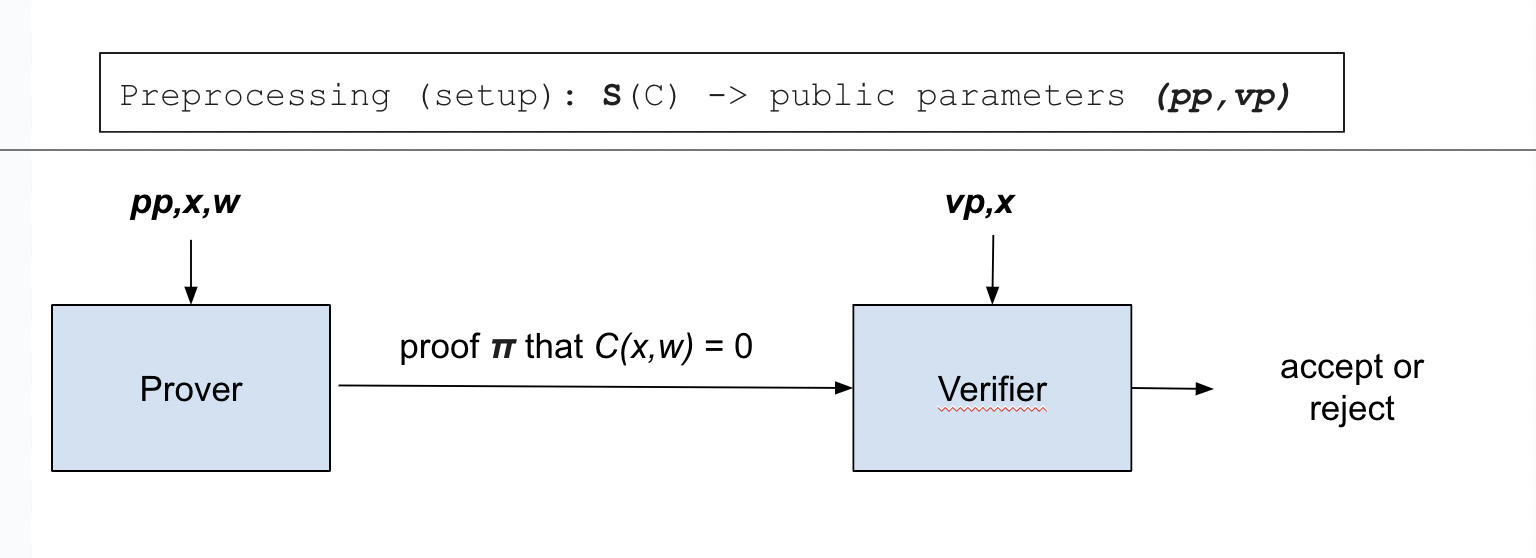
\includegraphics[width=130mm]{Circuit.png}
   \caption{Arithmetic circuit for SNARK \cite{ZKM2}}
   \label{overflow}
   \end{figure}


\begin{itemize}
\item \textbf{S(C)}: Public parameters (pp,vp) for prover and verifier
\item \textbf{P(pp,x,w)}: Proof $\pi$
\item \textbf{V(vp,x,$\pi$)}: Accept or reject
\item \textbf{C(x,w)}: Arithmetic circuit
\item \textbf{w}: Private witness
\item \textbf{x}: Public input
\end{itemize}
\fi

%-- TO REVIEW
\section{Proof of solvency}

A proof of solvency is a system where we prove that an entity, in most cases an exchange, holds enough assets to cover
the balance of every customer. In traditional finance, this would be done through an audit. While an audit can be useful,
it has many limitations. Obviously it requires the trust of another 3rd party, but it also poses a time constraint. Thus, it is impractical, even impossible
to hold an audit every single day, and in the Bitcoin world things move fast. It is essential to be able to fill a proof of solvency every single day.
The implementation of a mechanism to produce daily proofs of solvency is therefore of the utmost importance.

A proof of solvency is composed of a proof of assets, where we verify what assets the marketplace as control over, and the proof of liabilities,
where we confirm that the total amount of user deposits is smaller than the marketplaces assets.

The first paper about a proof of solvency focuses only on the proof of liabilities. In his paper Gregory Maxwell addresses the issue of verifying
the solvency of Bitcoin exchanges. \cite{chainlink_blog}
Maxwell's system ensures user privacy by maintaining confidentiality of individual account balances, while only revealing aggregate information in the proof of liabilities.
This is achieved through the application of Merkle trees.


\begin{figure}[H]
   \centering
   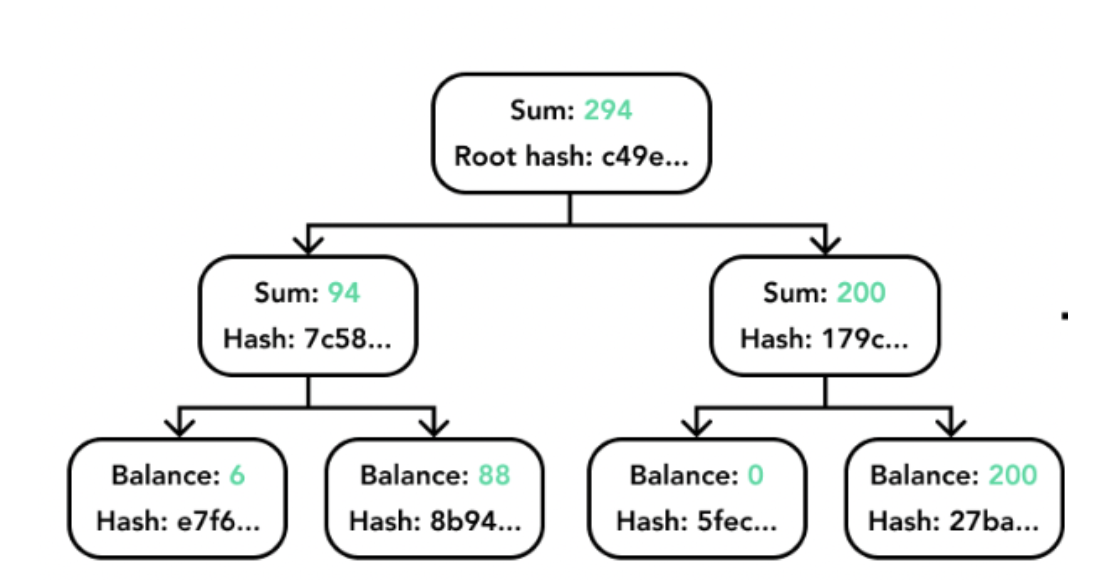
\includegraphics[width=130mm]{MerkleTreeLiabilities.png}
   \caption{Merkle tree for proof of liabilities}
   \label{overflow}
   \end{figure}


In the Merkle tree, every node contains a user's balance along with a hash-based commitment incorporating the customer ID and a nonce. The root of the tree is the sum of the balances.
To verify their inclusion in the total liabilities, users receive a subset of the hash tree from the exchange. This subset includes the user's nonce and the sibling nodes along the unique path from the user's leaf node to the root.
By comparing the received information to the exchange's broadcasted root node, users can confirm the inclusion of their balance.
While elegant, the protocol does have privacy implications. The exact value of the exchange's total liabilities, published in the root node, may be sensitive data.
Additionally, the proof of inclusion reveals the neighbor's balance, and the subtree's balance along the Merkle path.

The proof of liabilities is only part of the proof of solvency. A complete proof of solvency needs a proof of asset as well.
Provision describes the first preserving privacy proof of asset \cite{DBBBCC15}.

In Provisions, the focus shifts towards preserving privacy while still proving ownership of assets.
Instead of publicly demonstrating control over specific addresses, Provisions enables exchanges to prove ownership of an anonymous subset of addresses sourced from the blockchain.

Since these 2 papers, a lot of work was done to make the proof of solvency evolve. However, marketplaces still do not implement a proof of solvency, or a flawed and limited version of it.


\subsection{Real world proof of solvency}
In recent years, several major cryptocurrency exchanges, including Binance, Crypto.com, and Kraken, have taken steps to enhance transparency by provinding various proof of reserves.
Binance has implemented a proof of reserves system where they publish a monthly Merkle tree as their proof of liabilities, and disclose a list of their assets (every cryptocurrencies under their control) \cite{BPR}.
Crypto.com published a one-time audit \cite{CC22}.
Kraken is also publishing a proof of liabilities every few months, without a proof of assets. \cite{KK23}.

Although these proof of reserves may seem promising initially, they are primarily superficial.
The proofs have many shortcomings, they are not sufficient to prove that the marketplaces are solvent.
The first concern is the lack of proof of assets, or in Binance's case the lack of evidence demonstrating control over the wallets.
Without a reliable proof of assets, the proof of liabilities is worthless because it has nothing to compare against.

Moreover, the frequency of reporting is another area of concern. Given the dynamic nature of cryptocurrencies, a monthly report is not sufficient at all.
Binance is the only marketplace describing their proof of solvency, and we can see that it is not built with recurrence in mind.
The proof is created from scratch every time. They would need 150 servers to produce a daily proof \cite{BPS}.

















